\subsection{Les différentes vues}
\subsubsection{Liste des vues}
La plateforme est organisée selon une architecture MVC (Modèle - Vue - Contrôleur). Ainsi, les différents visuels/pages proposés (les vues) sont chacuns représentés par un fichier. Dans notre cas, ces fichiers sont situés dans le répertoire \texttt{telephonie/vue}. Nous allons dans un premier temps détailler la liste des vues, ces dernières seront ensuite présentées (fonctionnement et interraction avec les utilisateurs) dans les sous-sections suivantes.

Ainsi, l'application proposé au total sept vues :
\begin{itemize}
  \itemperso{Accueil}La page d'arrivée dans l'application qui présente uniquement les principaux objectifs de ce dernier. Ce visuel vous a été présenté à la Figure~\ref{fig:hello-world}.
  \itemperso{Téléphones}Cette page présente les différents téléphones proposés à la vente par Cenrale-Télécom. Elle permet au client de s'informer sur les modèles et de les acheter. Dans le même temps, elle permet à l'équipe administrative d'en référencer de nouveaux.
  \itemperso{Compte/Utilisateur}Ces vues permettent soit l'administration des utilisateurs par les administrateurs, soit à un client donné de consulter ses informations et de changer ses informations.
  \itemperso{Connexion}Une vue permet aux utilisateurs de se connecter/déconnecter.
  \itemperso{Factures}Cette vue n'est accessible qu'aux clients et permet à ces derniers de consulter leurs factures et de télécharger cette dernière au format PDF.
  \itemperso{Abonnements}Cette vue se décompose en trois vues intermédiaires :
  \begin{itemize}
    \subitemperso{Mes abonnements}Cette vue permet à un client de retrouver tous les abonnements auxquels il a souscrit, ainsi que les téléphones achetés chez Centrale-Télécom.
    \subitemperso{Vers l'étranger}Cette vue permet de préciser tous les abonnements étrangers proposés par Centrale-Télécom. Elle permet également aux administrateurs d'ajouter de nouveaux forfaits.
    \subitemperso{Formules}Cette vue permet de préciser toutes les formules proposées par Centrale-Télécom. Elle permet également aux administrateurs d'ajouter de nouvelles formules.
  \end{itemize}
\end{itemize}
Les spécificités par utilisateurs seront précisées plus en détails dans les sous-sections suivantes, ainsi que toutes les actions possibles.

\subsubsection{Navigation dans l'application}
Le dernier point général sur cette application est la navigation. Cette dernière est facilitée par un panneau latéral qui présente tous les menus de l'application. Dans le cas d'un client \og lambda\fg{}, on dispose du panneau latéral observable à la Figure~\ref{fig:navigation}.

\begin{figure}[ht]
  \centering
  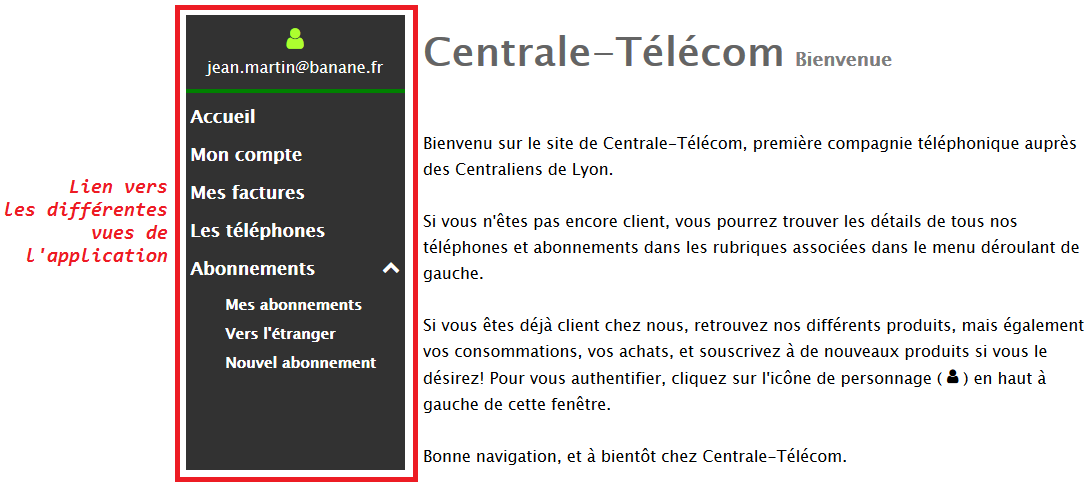
\includegraphics[width=.55\textwidth]{images/Plateforme/navigation}
  \caption{Panneau de navigation pour l'application}
  \label{fig:navigation}
\end{figure}

À moins d'être à l'accuel (cas de la Figure~\ref{fig:navigation}), la page courrante est surligné dans le volet de navigation pour que les utilisateurs sachent où ils se situent dans l'application.

%%% Local Variables:
%%% mode: latex
%%% TeX-master: "../../Rapport_BDD"
%%% End:
